% Semantic segmentation pipelines: encoder, U-Net decoder with two outputs, the line reconstruction of each output,
% and example results (thumbnails from fig:semantic-example and fig:center-line-method). Grid layout: four columns
% (x = 0, 3.7, 7.3, 10.9) and two rows (y = +-1.6); all thumbnails 30 mm wide, all process boxes 26 x 12 mm.
\begingroup
% Shared visual language for the three segmentation-method diagrams.
\tikzset{
    box/.style={draw, rounded corners=2pt, align=center, font=\small,
        text width=44mm, minimum height=9mm, inner sep=4pt, line width=0.5pt},
    process/.style={box, fill=gray!7},
    model/.style={box, very thick, fill=blue!5},
    output/.style={box, dashed},
    supervision/.style={box, densely dashed, fill=gray!7},
    link/.style={->, semithick},
    traininglink/.style={link, densely dashed}
}

\tikzset{
    box/.append style={font=\scriptsize, inner sep=3pt},
    stage/.style={font=\small\bfseries, anchor=south},
    thumb/.style={inner sep=0pt, draw=black!40, line width=0.3pt},
    thumbcap/.style={font=\scriptsize, align=center, text width=34mm, anchor=north, inner sep=2pt},
    recstep/.style={process, text width=31mm, minimum width=32mm, minimum height=16.4mm, inner sep=2pt},
}
\begin{tikzpicture}
    \def\xe{0}\def\xp{3.7}\def\xr{7.55}\def\xo{11.4}
    \def\ya{1.6}\def\yb{-1.6}
    % row a: text line mask
    \node[thumb] (ma) at (\xp,\ya) {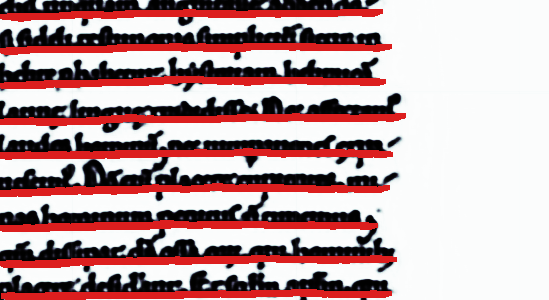
\includegraphics[width=30mm]{graphics/sem_ud_prob.png}};
    \node[thumbcap] (cma) at (ma.south) {1 class: text line probability,\\ARU-Net baselines (red)};
    \node[recstep] (ra) at (\xr,\ya) {\textbf{Projection cuts}\\[2pt]split the mask at\\projection valleys};
    \node[thumb] (oa) at (\xo,\ya) {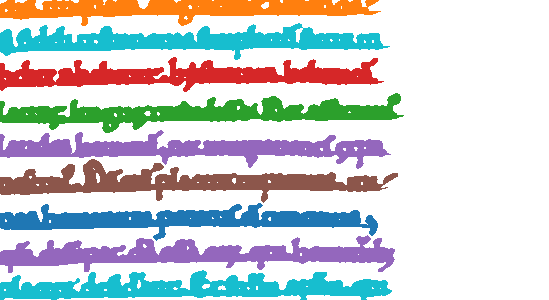
\includegraphics[width=30mm]{graphics/sem_ud_unet_lines.png}};
    \node[thumbcap] (coa) at (oa.south) {line instances};
    % row b: center lines
    \node[thumb] (mb) at (\xp,\yb) {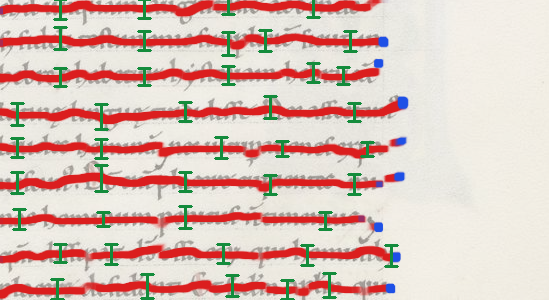
\includegraphics[width=30mm]{graphics/sem_ud_cl_maps.png}};
    \node[thumbcap] (cmb) at (mb.south) {4 classes: center, line end,\\distances up and down};
    \node[recstep] (rb) at (\xr,\yb) {\mbox{\textbf{Center-line decoding}}\\[2pt]join center lines, then\\ink ownership or BBox U-Net};
    \node[thumb] (ob) at (\xo,\yb) {
\includegraphics[width=30mm]{graphics/sem_ud_cl_lines.png}};
    \node[thumbcap] (cob) at (ob.south) {line instances};
    % U-Net decoder around both outputs, encoder with the same height
    \coordinate (dtop) at ($(ma.north)+(0,0.45)$);
    \begin{scope}[on background layer]
        \node[model, rounded corners=3pt, inner sep=4pt, fit=(dtop)(ma)(cma)(mb)(cmb)] (dec) {};
    \end{scope}
    \node[font=\scriptsize\bfseries, anchor=north] at ([yshift=-1.2mm]dec.north) {U-Net decoder};
    \node[model, rounded corners=3pt, inner sep=0pt, minimum width=20mm, fit={(\xe-1,0 |- dec.north) (\xe+1,0 |- dec.south)}] (enc) {};
    \node[align=center, font=\scriptsize] at (enc.center) {\textbf{Encoder}\\[2pt](Section~\ref{sec:backbones})};
    % headers on one baseline above the boxes
    \path (dec.north) ++(0,0.25) coordinate (hy);
    \node[stage] at (\xe,0 |- hy) {Encoder};
    \node[stage, align=center] at (\xp,0 |- hy) {Line\\prediction};
    \node[stage, align=center] at (\xr,0 |- hy) {Line\\reconstruction};
    \node[stage] at (\xo,0 |- hy) {Result};
    % arrows on the row centers
    \draw[link] (enc.east) -- (dec.west |- enc.east);
    \draw[link] (ma.east) -- (ra.west); \draw[link] (ra.east) -- (oa.west);
    \draw[link] (mb.east) -- (rb.west); \draw[link] (rb.east) -- (ob.west);
\end{tikzpicture}
\endgroup
